% ==========================================================================
% INFO 4617 Web Data Science -- Week 3: The Post-API Age (Chapter 3)
% Build:  latexmk -pdf week-03.tex   (from this folder; no env vars needed)
% (or run `make` from the slides/ directory to build every deck)
% ==========================================================================
\documentclass[9pt,aspectratio=169]{beamer}
% Resolve the shared theme/preamble in ../common/ when compiling this
% file directly from its own folder (no TEXINPUTS needed).
\makeatletter\def\input@path{{../common/}}\makeatother
% ==========================================================================
% Shared preamble for INFO 4617 Web Data Science weekly lecture decks
% Based on the Gotham beamer theme (vendored in this directory).
% Each week's slides.tex does:  % ==========================================================================
% Shared preamble for INFO 4617 Web Data Science weekly lecture decks
% Based on the Gotham beamer theme (vendored in this directory).
% Each week's slides.tex does:  % ==========================================================================
% Shared preamble for INFO 4617 Web Data Science weekly lecture decks
% Based on the Gotham beamer theme (vendored in this directory).
% Each week's slides.tex does:  \input{preamble}  (with common/ on TEXINPUTS)
% then sets \title/\subtitle/\author/\date and \begin{document}.
% ==========================================================================

\usetheme{gotham}

\usepackage{fbb}
\usepackage{booktabs}
\usepackage{graphicx}
\usepackage{tikz}
\usepackage{xcolor}
\usepackage{multirow}
\usepackage{listings}
\usetikzlibrary{positioning, arrows.meta, shapes}

% Bibliography
\usepackage[style=authoryear,
            backend=biber,
            maxcitenames=1,
            uniquename=false,
            uniquelist=false]{biblatex}
\addbibresource{bibliography.bib}

\gothamset{sectiontocframe default=off}

% ------------------------------------------------------------------ colors
\definecolor{cugold}{HTML}{CFB87C}
\definecolor{tab-red}{HTML}{E15759}
\definecolor{tab-orange}{HTML}{F28E2B}
\definecolor{tab-blue}{HTML}{4E79A7}
\definecolor{tab-cyan}{HTML}{76B7B2}
\definecolor{tab-green}{HTML}{59A14F}
\definecolor{tab-yellow}{HTML}{EDC948}
\definecolor{tab-purple}{HTML}{B07AA1}
\definecolor{tab-pink}{HTML}{FF9DA7}
\definecolor{tab-brown}{HTML}{9C755F}
\definecolor{tab-gray}{HTML}{BAB0AC}

\setbeamercolor{frametitle}{fg=black, bg=cugold}
\setbeamercolor{progress bar}{fg=cugold, bg=cugold!20}

\setbeamercolor{block title alerted}{fg=black, bg=cugold}
\setbeamercolor{block body alerted}{fg=black, bg=cugold!10}

% ------------------------------------------------------------------ footline
\setbeamertemplate{footline}{
  \begin{beamercolorbox}[wd=\paperwidth,ht=2.5ex,dp=1ex,right]{footline}
    {\footnotesize \insertframenumber{} of \inserttotalframenumber}
    \hspace*{2ex}
  \end{beamercolorbox}
}

% ------------------------------------------------------------------ helpers
\newcommand{\bottomcite}[1]{
    \vspace*{\fill}
    \vspace{-\baselineskip}
    {\tiny
    \rule{\textwidth}{0.3pt}\\
    #1
    }
    \vspace{0.5ex}
}

% Consistent code styling for the Wednesday "applied notebook" frames.
\lstdefinestyle{wds}{
    basicstyle=\ttfamily\scriptsize,
    keywordstyle=\color{tab-blue}\bfseries,
    commentstyle=\color{tab-green},
    stringstyle=\color{tab-orange},
    showstringspaces=false,
    breaklines=true,
    columns=fullflexible,
    language=Python,
    aboveskip=0.4em,
    belowskip=0.4em,
}
\lstset{style=wds}

% \dayband{Day}{Topic} -- a lightweight section divider label used to mark
% Monday / Wednesday / Friday within a week's deck.
\newcommand{\dayband}[2]{{\large\textbf{#1}}\;\textcolor{tab-gray}{\textbar}\;#2}
  (with common/ on TEXINPUTS)
% then sets \title/\subtitle/\author/\date and \begin{document}.
% ==========================================================================

\usetheme{gotham}

\usepackage{fbb}
\usepackage{booktabs}
\usepackage{graphicx}
\usepackage{tikz}
\usepackage{xcolor}
\usepackage{multirow}
\usepackage{listings}
\usetikzlibrary{positioning, arrows.meta, shapes}

% Bibliography
\usepackage[style=authoryear,
            backend=biber,
            maxcitenames=1,
            uniquename=false,
            uniquelist=false]{biblatex}
\addbibresource{bibliography.bib}

\gothamset{sectiontocframe default=off}

% ------------------------------------------------------------------ colors
\definecolor{cugold}{HTML}{CFB87C}
\definecolor{tab-red}{HTML}{E15759}
\definecolor{tab-orange}{HTML}{F28E2B}
\definecolor{tab-blue}{HTML}{4E79A7}
\definecolor{tab-cyan}{HTML}{76B7B2}
\definecolor{tab-green}{HTML}{59A14F}
\definecolor{tab-yellow}{HTML}{EDC948}
\definecolor{tab-purple}{HTML}{B07AA1}
\definecolor{tab-pink}{HTML}{FF9DA7}
\definecolor{tab-brown}{HTML}{9C755F}
\definecolor{tab-gray}{HTML}{BAB0AC}

\setbeamercolor{frametitle}{fg=black, bg=cugold}
\setbeamercolor{progress bar}{fg=cugold, bg=cugold!20}

\setbeamercolor{block title alerted}{fg=black, bg=cugold}
\setbeamercolor{block body alerted}{fg=black, bg=cugold!10}

% ------------------------------------------------------------------ footline
\setbeamertemplate{footline}{
  \begin{beamercolorbox}[wd=\paperwidth,ht=2.5ex,dp=1ex,right]{footline}
    {\footnotesize \insertframenumber{} of \inserttotalframenumber}
    \hspace*{2ex}
  \end{beamercolorbox}
}

% ------------------------------------------------------------------ helpers
\newcommand{\bottomcite}[1]{
    \vspace*{\fill}
    \vspace{-\baselineskip}
    {\tiny
    \rule{\textwidth}{0.3pt}\\
    #1
    }
    \vspace{0.5ex}
}

% Consistent code styling for the Wednesday "applied notebook" frames.
\lstdefinestyle{wds}{
    basicstyle=\ttfamily\scriptsize,
    keywordstyle=\color{tab-blue}\bfseries,
    commentstyle=\color{tab-green},
    stringstyle=\color{tab-orange},
    showstringspaces=false,
    breaklines=true,
    columns=fullflexible,
    language=Python,
    aboveskip=0.4em,
    belowskip=0.4em,
}
\lstset{style=wds}

% \dayband{Day}{Topic} -- a lightweight section divider label used to mark
% Monday / Wednesday / Friday within a week's deck.
\newcommand{\dayband}[2]{{\large\textbf{#1}}\;\textcolor{tab-gray}{\textbar}\;#2}
  (with common/ on TEXINPUTS)
% then sets \title/\subtitle/\author/\date and \begin{document}.
% ==========================================================================

\usetheme{gotham}

\usepackage{fbb}
\usepackage{booktabs}
\usepackage{graphicx}
\usepackage{tikz}
\usepackage{xcolor}
\usepackage{multirow}
\usepackage{listings}
\usetikzlibrary{positioning, arrows.meta, shapes}

% Bibliography
\usepackage[style=authoryear,
            backend=biber,
            maxcitenames=1,
            uniquename=false,
            uniquelist=false]{biblatex}
\addbibresource{bibliography.bib}

\gothamset{sectiontocframe default=off}

% ------------------------------------------------------------------ colors
\definecolor{cugold}{HTML}{CFB87C}
\definecolor{tab-red}{HTML}{E15759}
\definecolor{tab-orange}{HTML}{F28E2B}
\definecolor{tab-blue}{HTML}{4E79A7}
\definecolor{tab-cyan}{HTML}{76B7B2}
\definecolor{tab-green}{HTML}{59A14F}
\definecolor{tab-yellow}{HTML}{EDC948}
\definecolor{tab-purple}{HTML}{B07AA1}
\definecolor{tab-pink}{HTML}{FF9DA7}
\definecolor{tab-brown}{HTML}{9C755F}
\definecolor{tab-gray}{HTML}{BAB0AC}

\setbeamercolor{frametitle}{fg=black, bg=cugold}
\setbeamercolor{progress bar}{fg=cugold, bg=cugold!20}

\setbeamercolor{block title alerted}{fg=black, bg=cugold}
\setbeamercolor{block body alerted}{fg=black, bg=cugold!10}

% ------------------------------------------------------------------ footline
\setbeamertemplate{footline}{
  \begin{beamercolorbox}[wd=\paperwidth,ht=2.5ex,dp=1ex,right]{footline}
    {\footnotesize \insertframenumber{} of \inserttotalframenumber}
    \hspace*{2ex}
  \end{beamercolorbox}
}

% ------------------------------------------------------------------ helpers
\newcommand{\bottomcite}[1]{
    \vspace*{\fill}
    \vspace{-\baselineskip}
    {\tiny
    \rule{\textwidth}{0.3pt}\\
    #1
    }
    \vspace{0.5ex}
}

% Consistent code styling for the Wednesday "applied notebook" frames.
\lstdefinestyle{wds}{
    basicstyle=\ttfamily\scriptsize,
    keywordstyle=\color{tab-blue}\bfseries,
    commentstyle=\color{tab-green},
    stringstyle=\color{tab-orange},
    showstringspaces=false,
    breaklines=true,
    columns=fullflexible,
    language=Python,
    aboveskip=0.4em,
    belowskip=0.4em,
}
\lstset{style=wds}

% \dayband{Day}{Topic} -- a lightweight section divider label used to mark
% Monday / Wednesday / Friday within a week's deck.
\newcommand{\dayband}[2]{{\large\textbf{#1}}\;\textcolor{tab-gray}{\textbar}\;#2}


\title[Week 3 · Post-API Age]{{\Huge The Post-API Age}}
\subtitle{Week 3 · Foundations module · Textbook Chapter 3}
\author[Keegan]{\textbf{Brian C. Keegan, Ph.D.} \\ Associate Professor, Department of Information Science \\ University of Colorado Boulder}
\date{August 31, September 2 \& 4, 2026}

\begin{document}

\maketitle

% -------------------------------------------------------------------------
\begin{frame}{This week at a glance}
    \begin{columns}[T]
        \begin{column}{0.6\textwidth}
            The web used to invite us in. That has changed in recent year. 

            \bigskip
            
            \textit{Why} did this bargain change? \textit{How} can we keep doing public interest research anyway?

            \bigskip

            \dayband{Monday}{Concepts}
            \begin{itemize}\small
                \item The golden age
                \item Enclosure, exemption \& erosion
                \item Counter-values, lineages \& misconceptions
            \end{itemize}

            \medskip

            \dayband{Wednesday}{Notebook lab}
            \begin{itemize}\small
                \item Measure data access and forensic analysis of dead endpoints
            \end{itemize}

            \medskip

            \dayband{Friday}{Textbook revisions}
            \begin{itemize}\small
                \item Reviewing issues and proposing pull requests
            \end{itemize}
        \end{column}
        \begin{column}{0.35\textwidth}
            \begin{alertblock}{Monday lecture}
                \small Read Chapter 03 of the Web Data Science book
            \end{alertblock}
            \begin{alertblock}{Wednesday lab}
                \small Complete \textbf{Recommended Exercises}: fill in the empty cells, run everything, export to HTML, upload to Canvas by \textbf{Sunday 11:59pm}
            \end{alertblock}
            \begin{alertblock}{Friday notebook}
                \small You do not need to wait until Friday to begin to submit issues from textbook or notebook, upload link to issue by \textbf{Sunday 11:59pm}
            \end{alertblock}
        \end{column}
    \end{columns}
\end{frame}

% =========================================================================
\section{Monday · Concepts}
% =========================================================================

\begin{frame}{The golden age of web data access}
    \begin{columns}[T]
        \begin{column}{0.6\textwidth}
            Between roughly 2008 to 2018 the web was a mostly open that was easy(ish) to retrieve and analyze
            
            \medskip
            
            Websites rendered a mix of static and dynamic content
            
            \medskip
            
            Social platforms shared data: Twitter in 2006; Facebook in 2010; Reddit's API was free; Google exposed trends
            
            \medskip
            
            Platforms traded data access for lock-in to their ecosystems, credibility, recruitment
            
            \medskip
            
            This built my field of computational social science and a generation of data journalism and civic tech

            \medskip
            
            This is the ``API age'' $\rightarrow$ we're now in the ``post-API age''
        \end{column}
        \begin{column}{0.35\textwidth}\centering
            
\includegraphics[width=\textwidth]{slides/week-03/img/grandpa-simpson.jpg}
            {\scriptsize They just gave out data for free!}
        \end{column}
    \end{columns}

    \medskip

    \begin{block}{Three pressures}
        (1) Enclosure, (2) Exemption, (3) Erosion
    \end{block}
\end{frame}

\begin{frame}{Why platforms say no}
    \begin{columns}[T]
        \begin{column}{0.6\textwidth}
            Platforms invoke multiple reasons for restricting researcher access

            \medskip

            \begin{itemize}\small
                \item \textbf{Privacy \& safety.} User data can expose identities, enable harassment, or be repurposed in ways users never expected
                \item \textbf{Infrastructure.} Scraping and bulk API access impose real engineering and moderation costs
                \item \textbf{Business.} Data are an asset: competitors, AI companies, and researchers all want something the platform paid to collect
                \item \textbf{Legal risk.} Copyright, privacy law, contracts, and regulatory obligations make broad access risky
                \item \textbf{Control.} Platforms cannot easily distinguish public interest research from spam, surveillance, or commercial extraction
            \end{itemize}
        \end{column}
        \begin{column}{0.35\textwidth}
            \begin{alertblock}{The platform's questions}
                \small

                Who counts as a researcher?

                \medskip
                
                Access to what data?

                \medskip
                
                Under what rules?

                \medskip

                How does it help us?
            \end{alertblock}
        \end{column}
    \end{columns}
\end{frame}

\begin{frame}{Pressure 1 --- Enclosure}\small
    \begin{columns}[T]
        \begin{column}{0.6\textwidth}

            \textbf{Enclosure} privatizes a shared resource --- traces back to the fencing in of English common land. The data still exist, just on the other side of a paywall.
            \begin{itemize}\small
                \item \textbf{Twitter/X}: a free academic archive (2006--2021) $\rightarrow$ discontinued; enterprise access starts at \$42{,}000/month
                \item \textbf{Reddit}: free since 2008--2023 $\rightarrow$ \$0.24 per 1{,}000 calls; 7,000+ subreddit protests and Pushshift cut off
            \end{itemize}

            \medskip
            
            Two drivers:
            \begin{enumerate}
                \item \textbf{Independent scrutiny} --- researchers and journalists answering uncomfortable questions about polarization, harassment, privacy, financials, \textit{etc}.
                \item \textbf{AI training data} --- uncontaminated user-generated content becomes enormously valuable for training AI models
            \end{enumerate}
        \end{column}
        \begin{column}{0.35\textwidth}\centering
            \centering
            
\includegraphics[width=\textwidth]{slides/week-03/img/richmond-enclosure.jpg}\\
            {\scriptsize This land is my land now, it isn't your land anymore}
        \end{column}
    \end{columns}
\end{frame}

\begin{frame}{Pressure 2 --- Exemption}\small
    \begin{columns}[T]
        \begin{column}{0.6\textwidth}
            \textbf{Exemption}: platforms operate without transparency or accountability while surveilling and experimenting on you.

            \medskip

            From last week: when ``research'' appears in a TOS or Privacy Policy, it is generally permission for \textit{them} to do it to \textit{you}

            \medskip

            Researchers who want to hold platforms accountable get:
            
            \begin{itemize}\small
                \item cease-and-desist letters citing the Computer Fraud and Abuse Act
                \item NDA'd research collaborations
                \item data transparency delayed for years
                \item ``privacywashing'' and ``ethicswashing''
            \end{itemize}
            
        \end{column}
        \begin{column}{0.35\textwidth}\centering
            \centering
            
\includegraphics[width=\textwidth]{slides/week-03/img/meta-research-privacy.png}\\
            {\scriptsize Meta is suddenly very worried about privacy when researchers measure Meta behaving badly}
        \end{column}
    \end{columns}
\end{frame}

\begin{frame}{Pressure 3 --- Erosion}
    \begin{columns}[T]
        \begin{column}{0.6\textwidth}
            \textbf{Erosion} is the degradation in technology, practices, and other infrastructure that enables web data science.
            \begin{itemize}\small
                \item \textbf{Links rot.} About half the links in U.S. Supreme Court opinions are dead
                \item \textbf{Platforms churn.} GeoCities vanished; Parler disappears; Twitter became X
                \item \textbf{Sites redesign} and silently break every scraper
            \end{itemize}

            \smallskip

            For research this is a \textbf{reproducibility crisis}: data cannot be re-collected and analyses cannot be re-run $\rightarrow$ is it still science if it just worked one time for one team?
        \end{column}
        \begin{column}{0.35\textwidth}
            \centering
            
\includegraphics[width=\textwidth]{slides/week-03/img/scotus-link-rot.png}\\
            {\scriptsize SCOTUS decisions using broken links}
        \end{column}
    \end{columns}
\end{frame}

\begin{frame}{Counter-value 1 --- Openness against enclosure}
    \begin{columns}[T]
        \begin{column}{0.6\textwidth}
            \textbf{Openness}: conduct your own work so that it resists enclosure

            \medskip
            
            Document \textit{how} you collected: endpoints, parameters, dates, and the platform's constraints at collection time

            \medskip
            
            This documentation lets a future researcher understand your dataset after the source changes or vanishes

            \medskip
            
            Practice redundancy: deposit data in durable repositories (Zenodo, Dataverse, etc.), lean on the Internet Archive and Common Crawl, prefer openly licensed sources

            \medskip
            
            Wikipedia as the durable counter-factual --- open API, open license, full public dumps
            
        \end{column}
        \begin{column}{0.35\textwidth}
            \begin{alertblock}{Openness in one habit}
                \small Record the date. Preserve your data. Repeat to document changes.
            \end{alertblock}
        \end{column}
    \end{columns}
\end{frame}

\begin{frame}{Counter-value 2 --- Oversight against exemption}
    \begin{columns}[T]
        \begin{column}{0.6\textwidth}
            \textbf{Oversight}: consequential systems should be inspected by parties who do \textit{not} own them.

            \medskip
            
            Independent audits of platform algorithms and content moderation; documentation standards that make datasets and methods legible to review

            \medskip
            
            Regulation converts access from a favor into an obligation: EU DSA Article~40 compels vetted-researcher access to very large platforms
        \end{column}
        \begin{column}{0.35\textwidth}
            \begin{alertblock}{This course is oversight}
                \small Someone who can retrieve, parse, and analyze web data independently is someone who can hold platforms accountable instead of asking politely
            \end{alertblock}
        \end{column}
    \end{columns}
\end{frame}

\begin{frame}{Counter-value 3 --- Ownership against erosion}
    \begin{columns}[T]
        \begin{column}{0.6\textwidth}
            \textbf{Ownership}: prefer arrangements where communities govern the infrastructure their data lives in rather than trusting someone else will keep it running forever

            \medskip
            
            Federated systems on open protocols distribute control: no single acquisition or pricing decision can enclose the whole network
            \begin{itemize}
                \item HTTP, torrents, RSS, Mastodon, Bluesky, \textit{etc}.
            \end{itemize}

            \medskip
            
            Community archives, data cooperatives, and volunteer efforts hold collective traces collectively
            
        \end{column}
        \begin{column}{0.35\textwidth}
            \begin{alertblock}{The trade}
                \small Federation exchanges convenience for control: smaller populations, uneven moderation, more work per query
            \end{alertblock}
        \end{column}
    \end{columns}
\end{frame}

\begin{frame}{Myths}
    \begin{columns}[T]
        \begin{column}{0.6\textwidth}
            Five common beliefs. For each, commit: \textbf{true or false?}
            \begin{enumerate}
                \item ``The post-API age means APIs are gone.''
                \item ``If the API closes, I'll just scrape.''
                \item ``If data is publicly, collecting it is permitted.''
                \item ``This only matters for social media research.''
                \item ``Nothing can be done about it.''
            \end{enumerate}
        \end{column}
        \begin{column}{0.35\textwidth}
            \begin{alertblock}{Rules}
                \small Write your five answers down first; then we take a hand count, myth by myth. Defend your minority votes --- some of these are \textit{almost} true.
            \end{alertblock}
        \end{column}
    \end{columns}
\end{frame}

\begin{frame}{Myth busting}
    \begin{enumerate}
        \item \textbf{APIs are everywhere.} More exist than ever; what is disappearing is \textit{free access for outside observers}, replaced by paid tiers, gated programs, and licensing deals
        \item \textbf{Scraping is one tool in a portfolio.} Legal risks are changing but non-zero, adversarial site design, poor scalability
        \item \textbf{Visibility, permission, and ethics are three different questions} A public post's author may never have expected a dataset; a viewable page's ToS may forbid automated collection
        \item \textbf{Enclosure follows AI-training value} wherever it appears: news archives, code repositories, forums, image libraries. Government data stays open by legal mandate
        \item \textbf{The environment is contested.} Regulation is creating access obligations, archives are institutionalizing preservation, and federated alternatives are growing
    \end{enumerate}
\end{frame}

\begin{frame}{Other professions and disciplines}
    \begin{columns}[T]
        \begin{column}{0.6\textwidth}
            \textbf{Public interest data science} asks how technical skills can increase the public's capacity to know, scrutinize, and act on consequential institutions and systems.

            \medskip

            Retrieving data is never only a technical problem:

            \begin{itemize}\small
                \item \textbf{Access} --- who can observe powerful institutions
                \item \textbf{Methods} --- what can be made visible and auditable
                \item \textbf{Infrastructure} --- whether evidence remains available
                \item \textbf{Practice} --- who benefits from our technical work
            \end{itemize}

        Other professions have met the problem of powerful actors controlling information the public needs.
        
        \end{column}

        \begin{column}{0.35\textwidth}
            \begin{alertblock}{Five older traditions}
                \small
                Other flavors of public interest

                \medskip

                \textbf{Journalism} --- scrutiny

                \textbf{Law} --- compelled disclosure

                \textbf{Accounting} --- independent audit

                \textbf{Urban planning} --- participation

                \textbf{Engineering} --- public safety
            \end{alertblock}
        \end{column}
    \end{columns}

    \bigskip

    \begin{alertblock}{The point}
        \small
        Not one definition of ``the public good,'' but traditions for making power observable, reviewable, and contestable.
    \end{alertblock}
\end{frame}

\begin{frame}{Lineage 1 --- Journalism}
    \begin{columns}[T]
        \begin{column}{0.6\textwidth}
            Journalism is not just inspiration for public interest data science; it is an older professional technology for working with contested evidence.

            \medskip

            \textbf{FOIA and state records laws} turn watchdog work from a polite request into a procedural right: deadlines, exemptions, appeals, and records that agencies did not voluntarily publish.

            \medskip

            \textbf{Verification and provenance} are default practices: a claim must trace back to a source, a document, a row, or an interview.

            \medskip

            \textbf{Right of reply} treats the target of an investigation as part of the verification process, not as a veto-holder.

            \medskip

            \textbf{Collaborative investigations} scale
            scrutiny beyond any one newsroom.
        \end{column}
        \begin{column}{0.35\textwidth}
            \begin{alertblock}{Data science echo}
                \small
                Journalism's lesson is procedural:

                \medskip

                show your work, preserve provenance, invite challenge, publish under pressure
            \end{alertblock}
        \end{column}
    \end{columns}
\end{frame}

\begin{frame}{Lineage 2 --- Law}
    \begin{columns}[T]
        \begin{column}{0.6\textwidth}
            Law contributes procedures for extracting evidence from institutions that have incentives not to disclose it.

            \medskip

            \textbf{Public-records law} creates a statutory geometry: request, deadline, exemption, appeal, litigation.

            \medskip

            \textbf{Discovery} compels records, testimony, and interrogatory answers that no public API or FOIA request would expose.

            \medskip

            \textbf{Cause lawyering} treats a case as a way to change a rule, not merely resolve one dispute.

            \medskip

            \textbf{Sandvig v. Barr} matters because it reduced the CFAA chill around audit studies that
            use bots, paired accounts, or ToS-violating methods.
        \end{column}
        \begin{column}{0.35\textwidth}
            \begin{alertblock}{Data science echo}
                \small
                Legal infrastructure before technical accountability can begin:

                \medskip

                requests, complaints, briefs, subpoenas, protective orders.
            \end{alertblock}
        \end{column}
    \end{columns}
\end{frame}

\begin{frame}{Lineage 3 --- Accounting}
    \begin{columns}[T]
        \begin{column}{0.6\textwidth}
            Accounting contributes the machinery for making claims credible to other institutions.

            \medskip

            \textbf{Audits} create an independent record of what was checked, how, and against which standards.

            \medskip

            \textbf{Materiality} distinguishes errors that matter from noise: not every discrepancy changes the public claim.

            \medskip

            \textbf{Workpapers} make the audit inspectable: evidence, judgment calls, sampling choices, and reviewer sign-off.

            \medskip

            \textbf{Standardized reporting} makes one organization's claims comparable to another's.
        \end{column}
        \begin{column}{0.35\textwidth}
            \begin{alertblock}{Data science echo}
                \small
                Datasheets, model cards, replication packages, pinned environments, and audit logs
                are early versions of inspectability.
            \end{alertblock}
        \end{column}
    \end{columns}
\end{frame}

\begin{frame}{Lineage 4 --- Urban planning}
    \begin{columns}[T]
        \begin{column}{0.6\textwidth}
            Affected publics: technical decisions are also decisions about land, exposure, mobility, housing, and political voice.

            \medskip

            \textbf{Environmental impact statements} force agencies to document consequences before irreversible action.

            \medskip

            \textbf{Public comment} creates a record, but not necessarily power: consultation can become participation theater.

            \medskip

            \textbf{Stakeholder maps} make visible who is in the room, who is affected, who has formal authority, and who has remedy.
            
        \end{column}
        \begin{column}{0.35\textwidth}
            \begin{alertblock}{Data science echo}
                \small
                Disclose before deployment, map affected parties, document expected harms, and create a record for challenge.
            \end{alertblock}
        \end{column}
    \end{columns}
\end{frame}

\begin{frame}{Lineage 5 --- Engineering}
    \begin{columns}[T]
        \begin{column}{0.6\textwidth}
            Technical practitioners have public duties that can override duties to clients or employers.

            \medskip

            \textbf{Licensure} gives some practitioners standing to refuse unsafe work.

            \medskip

            \textbf{Codes and standards} convert past failures into shared constraints on future design.

            \medskip

            \textbf{Ethics canons} name the public as a client even when the public did not sign the contract.

            \medskip

            \textbf{Failure analysis} treats accidents as institutional evidence with required investigation and disclosure
        \end{column}
        \begin{column}{0.35\textwidth}
            \begin{alertblock}{Data science echo}
                \small
                Data science has no equivalent license to lose, no universally enforced canon, and no mature failure-reporting regime.
            \end{alertblock}
        \end{column}
    \end{columns}
\end{frame}

\begin{frame}{Pushback 1 --- Sue over the gate}
    \begin{columns}[T]
        \begin{column}{0.6\textwidth}
            Researchers have challenged the idea that platform terms alone should define the boundary of legitimate inquiry.

            \medskip

            \begin{itemize}\small
                \item \textbf{Sandvig v. Sessions/Barr.} Civil-rights researchers challenged CFAA risk around audit studies using bots, scraping, and tester accounts
                \item \textbf{Van Buren aftermath.} Terms-of-service violations alone are a weaker basis for treating research as ``hacking''
                \item \textbf{Strategic target.} The point is reducing the legal chill around public interest auditing
            \end{itemize}
        \end{column}
        \begin{column}{0.35\textwidth}
            \begin{alertblock}{The legal move}
                \small
                Can researchers test platforms the way civil-rights testers test landlords, lenders, or employers?
            \end{alertblock}
        \end{column}
    \end{columns}
\end{frame}

\begin{frame}{Pushback 2 --- Build around the missing API}
    \begin{columns}[T]
        \begin{column}{0.6\textwidth}
            Build research capacity outside of platforms with technical infrastructure you control

            \medskip

            \begin{itemize}\small
                \item \textbf{Platform research tools.} Meta Content Library/API, TikTok Research API, controlled-access clean rooms
                \item \textbf{Independent archives.} Internet Archive, Common Crawl, End-of-Term archives, local WARC collections
                \item \textbf{User-side collection.} Data donations, browser instrumentation, panels, screen capture, audit accounts
                \item \textbf{Shared infrastructure.} Replication packages, codebooks, documented missingness, synthetic examples
            \end{itemize}

            \medskip

            Major trade-offs with comprehensiveness, reliability, resolution
        \end{column}
        \begin{column}{0.35\textwidth}
            \begin{alertblock}{New access model}
                \small
                Move from a single point of failure to archives + enclaves + donations + audits
            \end{alertblock}
        \end{column}
    \end{columns}
\end{frame}

\begin{frame}{Pushback 3 --- Turn access into a policy problem}
    \begin{columns}[T]
        \begin{column}{0.6\textwidth}
            Researchers also push by making platform access a matter of public obligation, not platform generosity.

            \medskip

            \begin{itemize}\small
                \item \textbf{EU: DSA Article 40.} Vetted researchers can seek public or non-public VLOP/VLOSE data
                \item \textbf{Federal proposals.} Researcher requests require ad libraries, moderation stats, and recommender data
                \item \textbf{State transparency laws.} California AB 587 seek disclosure, but 1A challenges narrow what states can compel
                \item \textbf{Public officials on private platforms.} FOIA, state public-records laws, and 1A doctrine can turn official accounts into transparency targets
            \end{itemize}

        \medskip

        Public power in private infrastructure still deserves public oversight.
        \end{column}
        \begin{column}{0.35\textwidth}

            
\includegraphics[width=\textwidth]{slides/week-03/img/eu-gpt-reddit-roblox.jpeg}
        \end{column}
    \end{columns}
\end{frame}

\begin{frame}{Activity --- Platform vs. researcher hidden profile negotiation}
    \begin{columns}[T]
        \begin{column}{0.48\textwidth}
            \begin{alertblock}{Researchers}
                \small
                If your birthday is an even day, you are a naughty researcher trying to get platform data for evil

                \medskip

                If your birthday is an odd day, you are a nice researcher trying to get platform data for good

                \medskip

                \textbf{Records} --- posts, users, comments, ads, algorithms?

                \medskip

                \textbf{Fields} --- text, timestamps, engagement, deletions?

                \medskip

                \textbf{History} --- how far back? how often?
            \end{alertblock}
        \end{column}

        \begin{column}{0.48\textwidth}
            \begin{alertblock}{Platform operators}
                \small
                
                If your birthday is an even day, you are a naughty platform trying to protect platform data for evil

                \medskip

                If your birthday is an odd day, you are a nice platform trying to protect platform data for good

                \medskip

                \textbf{Privacy} --- could users be identified or harmed?

                \medskip

                \textbf{Revenue} --- are you giving away a valuable asset?

                \medskip

                \textbf{Infrastructure} --- what does bulk access cost?

                \medskip

                \textbf{Competition} --- could others copy products or models?

                \medskip

                \textbf{Legal risk} --- copyright, contracts, regulators, lawsuits?
            \end{alertblock}
        \end{column}
    \end{columns}

    \bigskip
    Enclosure vs. openness; Exemption vs. oversight; Erosion vs. ownership and appeals to public interest
    
\end{frame}


\begin{frame}{Debrief --- What did access cost?}
    \begin{columns}[T]
        \begin{column}{0.55\textwidth}
        
            Summarize your deal.

            \medskip

            1. What did the researchers originally ask for?

            \medskip

            2. What did the platform actually agree to provide?

            \medskip

            3. What restriction was hardest to negotiate?

            \medskip

            4. What did you trade away to get access?

            \medskip

            5. Reproducible by other parties?

        \bigskip
        \end{column}

        \begin{column}{0.4\textwidth}

            \begin{center}
                \resizebox{\linewidth}{!}{%
                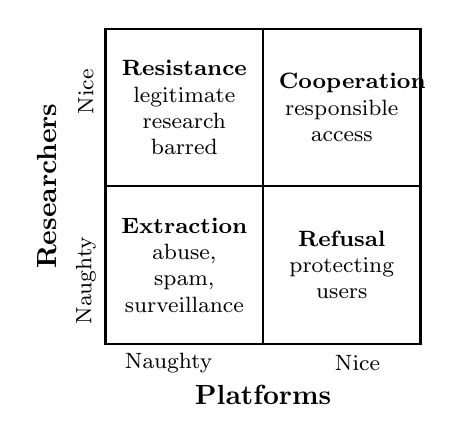
\begin{tikzpicture}
                    % Grid
                    \draw[thick] (0,0) rectangle (4,4);
                    \draw[thick] (2,0) -- (2,4);
                    \draw[thick] (0,2) -- (4,2);
                
                    % Axis labels
                    \node[font=\bfseries] at (2,-0.65) {Platforms};
                    \node[font=\footnotesize] at (0.8,-0.25) {Naughty};
                    \node[font=\footnotesize] at (3.2,-0.25) {Nice};
                
                    \node[font=\bfseries,rotate=90] at (-0.75,2) {Researchers};
                    \node[font=\footnotesize,rotate=90] at (-0.25,0.8) {Naughty};
                    \node[font=\footnotesize,rotate=90] at (-0.25,3.2) {Nice};
                
                    % Quadrants
                    \node[align=center,font=\footnotesize,text width=1.6cm] at (1,3) {
                        \textbf{Resistance}\\
                        legitimate research barred
                    };
                
                    \node[align=center,font=\footnotesize,text width=1.6cm] at (3,3) {
                        \textbf{Cooperation}\\
                        responsible access
                    };
                
                    \node[align=center,font=\footnotesize,text width=1.6cm] at (1,1) {
                        \textbf{Extraction}\\
                        abuse, spam,\\
                        surveillance
                    };
                
                    \node[align=center,font=\footnotesize,text width=1.6cm] at (3,1) {
                        \textbf{Refusal}\\
                        protecting users
                    };
                \end{tikzpicture}%
                }
                \end{center}

        \end{column}
    \end{columns}
\end{frame}

\begin{frame}{Wednesday: measure it, then take it home}
    \begin{columns}[T]
        \begin{column}{0.6\textwidth}
            Build an access matrix: probe eight live endpoints with no credentials and tabulate who answers, who refuses, and how
            
            \medskip
            
            Run dead-endpoint forensics: autopsies of Pushshift, CrowdTangle, and Twitter v1.1 --- three retirements, three different failure signatures
        \end{column}
        \begin{column}{0.35\textwidth}
            \begin{alertblock}{Take-home: the 7-step audit}
                \footnotesize
                \begin{enumerate}\footnotesize
                    \item Named \texttt{User-Agent}
                    \item Probe one endpoint by hand
                    \item All eight $\rightarrow$ dated DataFrame
                    \item Add two endpoints \textit{you} care about
                    \item Diagnose one refusal, attribute it
                    \item Autopsy one retired endpoint
                    \item Write up what changed
                \end{enumerate}
            \end{alertblock}
        \end{column}
    \end{columns}
\end{frame}

% =========================================================================
\section{Wednesday · Notebook Lab}
% =========================================================================

\begin{frame}[fragile]{Claims you can check --- the access matrix}
    Enclosure, exemption, and erosion are claims about the world. Claims about the world can be checked. The chapter's audit asks eight endpoints one question: \textit{if I show up with no credentials, what happens?}
\begin{lstlisting}
def probe(name, url):
    """Ask one endpoint for data without credentials; describe the answer."""
    try:
        response = requests.get(url, headers=HEADERS, timeout=20)
    except requests.RequestException as error:   # no answer is a result too
        return {"api": name, "status": None, "verdict": "unreachable"}
    verdict = ("open" if response.status_code == 200
               else "gated" if response.status_code in (401, 403) else "other")
    return {"api": name, "status": response.status_code, "verdict": verdict,
            "content_type": response.headers.get("content-type", "")}
\end{lstlisting}
    \small Measured 28 Aug 2026: Wikipedia, Hacker News, arXiv, Mastodon, Bluesky \textbf{open}; Reddit and X \textbf{gated}; Meta Graph refuses without a token. Your run \textit{will} differ --- that is the finding, so record the date.
\end{frame}

\begin{frame}{Read the rows, not the totals}
    \begin{columns}[T]
        \begin{column}{0.6\textwidth}
            The useful information is in the differences:
            \begin{itemize}\small
                \item \textbf{Wikipedia, Hacker News, arXiv} answer anonymous requests with data, and have for a decade --- a non-profit, an incubator, a university consortium. No one here monetizes attention.
                \item \textbf{Reddit}: status 403, content-type \texttt{text/html} --- not an API refusing you, a \textit{block page} served where JSON lived from 2008 to 2023. Enclosure is a content-type header.
                \item \textbf{X}: \texttt{401 application/problem+json} --- a machine-readable, honest refusal. Differently built gates tell you whether applying for access would even help.
            \end{itemize}
        \end{column}
        \begin{column}{0.35\textwidth}
            \begin{alertblock}{Attribute before you conclude}
                \footnotesize While the chapter was drafted, GitHub returned 403 --- a striking finding, since GitHub allows 60 anonymous requests/hour. The \textit{body} named the drafting sandbox, not GitHub. Check \texttt{server} and \texttt{via}, read the body, retest from a second network.
            \end{alertblock}
        \end{column}
    \end{columns}
    \bottomcite{Textbook Ch.~3, ``Reading the Failure, Not Just the Status Code.'' A measurement that describes your instrument is worse than none.}
\end{frame}

\begin{frame}{Dead-endpoint forensics --- three ways to die}
    \begin{columns}[T]
        \begin{column}{0.6\textwidth}
            How a retired endpoint refuses tells you whether anything can be recovered:
            \begin{itemize}\small
                \item \textbf{Pushshift} answers \texttt{403} in JSON: \texttt{\{"detail": "Not authenticated"\}}. \textbf{Gated, not gone} --- it still runs, for Reddit moderators. A gated service can be negotiated with.
                \item \textbf{CrowdTangle} does not resolve at all. No HTTP conversation happens. \textbf{Enclosure completed}; nothing left to ask.
                \item \textbf{Twitter v1.1} parses your request and rejects it (error 215). Alive, serving paying customers. \textbf{Repriced, not removed.}
            \end{itemize}
        \end{column}
        \begin{column}{0.35\textwidth}
            \begin{block}{The archive keeps the receipts}
                \footnotesize Wayback's last captures: \texttt{api.pushshift.io} --- 25 May 2023, six weeks before Reddit's pricing took effect. \texttt{crowdtangle.com} --- 14 Aug 2024, the month Meta retired it. The shutdowns are written in the archival record.
            \end{block}
            {\scriptsize Archived docs are how you reconstruct what a five-year-old paper's dataset contained. More in Ch.~7.}
        \end{column}
    \end{columns}
    \bottomcite{Textbook Ch.~3, ``Dead-Endpoint Forensics.'' Always pass \texttt{timeout=} --- a dead host may drop packets rather than refuse.}
\end{frame}

\begin{frame}{The take-home --- a guided audit in seven steps}
    \begin{columns}[T]
        \begin{column}{0.6\textwidth}
            The notebook's \textbf{Recommended Exercises} walk the audit end to end. Fill in each empty cell:
            \begin{enumerate}\small
                \item Define \texttt{HEADERS} with your named User-Agent
                \item Probe \textbf{one} endpoint by hand; look at the answer
                \item Build the eight-endpoint matrix as a DataFrame
                \item Add \textbf{two} endpoints you might actually study
                \item Diagnose one refusal: \texttt{server}, \texttt{via}, body
                \item Autopsy one retired endpoint: gone, gated, or repriced?
                \item Interpret: what differed from the book, and why?
            \end{enumerate}
        \end{column}
        \begin{column}{0.35\textwidth}
            \begin{block}{Submitting}
                \footnotesize Run all cells, then export: \textit{File $\rightarrow$ Save and Export Notebook As $\rightarrow$ HTML}. Upload the \texttt{.html} file to Canvas by \textbf{Sunday 11:59pm}. Canvas accepts only \texttt{.html} --- code and output together, as executed.
            \end{block}
            {\scriptsize Start in class, finish at home. Work in pairs; submit your own run.}
        \end{column}
    \end{columns}
    \bottomcite{Textbook Ch.~3, Recommended Exercises. Date-stamp your matrix --- it is a snapshot, not a fact.}
\end{frame}

\begin{frame}{If you finish early --- the additional exercises}
    \begin{columns}[T]
        \begin{column}{0.6\textwidth}
            The chapter's \textbf{Additional Exercises} are optional, open-ended extensions --- worth your time, not required:
            \begin{enumerate}\small
                \item \textbf{Extend the autopsy} --- two more retired endpoints: gone, gated, or repriced, and who is left to ask?
                \item \textbf{Timeline} --- five API-access events, three platforms, 2008 to today; tag each with its pressure.
                \item \textbf{Framework application} --- 500 words on a platform change \textit{not} in the chapter.
                \item \textbf{Contingency plan} --- a project on one source, plus three fallbacks if it vanishes mid-study.
                \item \textbf{Public interest audit} --- how would current restrictions hit a real API-enabled project?
                \item[6.] \textbf{5617}: read \textcite{davidson2023platform} and \textcite{perriam2020digital}; write a 2--3 page research-access brief for one platform.
            \end{enumerate}
        \end{column}
        \begin{column}{0.35\textwidth}
            \begin{block}{Fallbacks worth knowing}
                \footnotesize Official research programs (real but rationed) $\cdot$ data donation $\cdot$ FOIA / records requests (Ch.~11) $\cdot$ crowdsourcing.
            \end{block}
            \begin{block}{Show-and-Tell}
                \footnotesize Bring one: an access change that surprised you, a dataset you fear losing, or a question for a research design.
            \end{block}
        \end{column}
    \end{columns}
    \bottomcite{Textbook Ch.~3, Additional Exercises \& ``What This Means for Practice.''}
\end{frame}

\begin{frame}[fragile]{Openness in practice --- document the collection}
    The audit teaches you to date-stamp a measurement; openness generalizes that habit. Record \textbf{what} you collected and also \textbf{how}: endpoints, parameters, dates, and the platform's constraints \parencite{gebru2021datasheets}. A future reader (or you, in a year) can then reconstruct exactly what was allowed:
\begin{lstlisting}
collection = {
    "source":      "reddit.com  (PRAW, r/ClimateChange)",
    "endpoint":    "GET /r/{sub}/top   params: t=year, limit=1000",
    "collected":   "2026-02-14",
    "access_tier": "researcher program (application-gated)",
    "constraints": "no redistribution of raw comments; 100 req/min",
    "known_gaps":  "pre-2023 history unavailable -- Pushshift offline",
}
import json, pathlib
pathlib.Path("datasheet.json").write_text(json.dumps(collection, indent=2))
# The datasheet travels next to the data; the source may change, the record does not.
\end{lstlisting}
    \bottomcite{Textbook Ch.~3, ``Openness'' --- documentation as the practice that survives enclosure.}
\end{frame}

\begin{frame}[standout]
    ``If the API closes, I'll just scrape.''\\[0.6em]
    {\large Visibility, permission, and ethics are three different questions.}\\[1em]
    Scraping is one tool in a portfolio ---\\
    not an escape hatch that makes enclosure irrelevant.
\end{frame}

% =========================================================================
\section{Friday · Textbook Revisions}
% =========================================================================

\begin{frame}{Improving Chapter 3 together}
    \begin{columns}[T]
        \begin{column}{0.6\textwidth}
            Last week you filed an \textbf{issue} --- a report that something is wrong. Today you take the next step and propose the \textbf{fix} itself: your \textbf{first pull request}, against \texttt{ch-03-post-api.qmd}, plus reviews of two classmates'.

            \bigskip

            The workflow, in GitHub Desktop or \texttt{gh} (no raw \texttt{git} needed):
            \begin{enumerate}\small
                \item \textbf{Clone} the book repo, then create a \textbf{branch}
                \item Edit the chapter; \textbf{commit} with a clear message
                \item \textbf{Push}, then open a PR describing \textit{what} and \textit{why}
                \item Review two peers' PRs: kind, specific, actionable
            \end{enumerate}

            \medskip

            This is a \textbf{fast-moving} chapter --- prices, lawsuits, and regulations change monthly --- so it always needs hands.
        \end{column}
        \begin{column}{0.35\textwidth}
            \centering
            
\includegraphics[width=\textwidth]{img/pr_review.png}
        \end{column}
    \end{columns}
    \bottomcite{Contributions \& reviews count toward the Textbook Revisions grade (15\%).}
\end{frame}

\begin{frame}{A revision menu for Chapter 3}
    High-value targets --- pick one and scope it to a single PR:
    \begin{itemize}\small
        \item \textbf{Add the missing figures.} The chapter still has no figures. Contribute a three-pressures diagram, an API-access timeline (2008--2026), or a link-rot chart --- the deck's placeholders show the need.
        \item \textbf{Re-run the audit.} The access matrix and forensics outputs are dated 28 Aug 2026 and \textit{will} drift. Re-run the chapter's code, and where a row changed, update the printed output and the prose that reads it. This is the chapter's built-in revision engine.
        \item \textbf{Update the moving numbers.} Verify and re-cite the Twitter/X pricing, the Reddit--Google deal, and DSA Article~40's implementation status ``as of mid-2026.'' Flag what has gone stale.
        \item \textbf{Resolve the editorial TODOs.} The source carries author-voice and ``add citation when published'' notes (the openness/oversight/ownership framing). Track down a source or draft the text.
        \item \textbf{Extend a Misconception or Further Reading.} Add a post-2023 source on AI-training licensing, tied to ``enclosure logic is spreading.''
        \item \textbf{Verify the cross-references.} Ch.~3 leans on many \texttt{@sec-} links (ethics, wikipedia, archives, automation, social, government). Confirm each resolves and is described accurately.
    \end{itemize}
    \bottomcite{Targets drawn from the chapter's callouts, thin exercises, ``Common Misconceptions,'' and ``Further Reading.''}
\end{frame}

\begin{frame}{A good revision, and a good review}
    \begin{columns}[T]
        \begin{column}{0.6\textwidth}
            \begin{block}{A strong PR}
                \begin{itemize}\small
                    \item One focused change, clearly titled
                    \item Explains the problem it fixes
                    \item Builds (\texttt{quarto render}) without errors
                    \item Matches the book's voice and notation
                    \item Discloses any AI assistance
                \end{itemize}
            \end{block}
        \end{column}
        \begin{column}{0.35\textwidth}
            \begin{block}{A strong review}
                \begin{itemize}\small
                    \item Runs / reads the change, not just skims
                    \item Names specifics (line, claim, source)
                    \item Separates ``must fix'' from ``nice to have''
                    \item Is generous --- assume good faith
                    \item Ends with a clear verdict
                \end{itemize}
            \end{block}
        \end{column}
    \end{columns}
    \medskip
    \centering\small Next week: \textbf{Data formats} --- XML \& JSON, the shapes web data actually arrives in.
\end{frame}

% =========================================================================
\begin{frame}{Key takeaways}
    \begin{enumerate}
        \item The open-API era ($\sim$2008--2018) was a \textbf{strategic bargain}, not a natural state --- and computational social science was built on the trade.
        \item \textbf{Enclosure} converts collective data into private assets: shutdowns, repricing, and AI-training licensing deals.
        \item \textbf{Exemption} is the asymmetry of scrutiny --- platforms study users freely while blocking those who study platforms.
        \item \textbf{Erosion} is infrastructural decay, so reproducibility is a problem you must solve \textit{at collection time}.
        \item \textbf{Access is measurable, not just arguable} --- an unauthenticated probe places a platform on the open-to-closed gradient today, and \textit{how} a dead endpoint refuses tells you whether anyone is left to negotiate with.
        \item The response is \textbf{redundancy}: openness, oversight, ownership --- and mastery of many access techniques so no single closure ends your research.
    \end{enumerate}
    \medskip
    \bottomcite{Reading: Textbook Ch.~3. See \textcite{freelon2018computational}; \textcite{bruns2019after}; \textcite{lazer2020computational}.}
\end{frame}

\end{document}
